\section{Consignes de présentation/Presentation guidelines}
\label{chap:consignes}

\selectlanguage{french}
Vous venez de télécharger la classe personnalisée LaTeX AMU pour les thèses de doctorat de l'université d'Aix-Marseille.
Certains éléments doivent obligatoirement être utilisés:

\selectlanguage{english}
You have downloaded the LaTeX AMU custom class for Aix-Marseille University doctoral theses.
Some elements must be used:
\\


\begin{figure}[h!tbp]
	%\vspace{0.5cm}
	\centering
	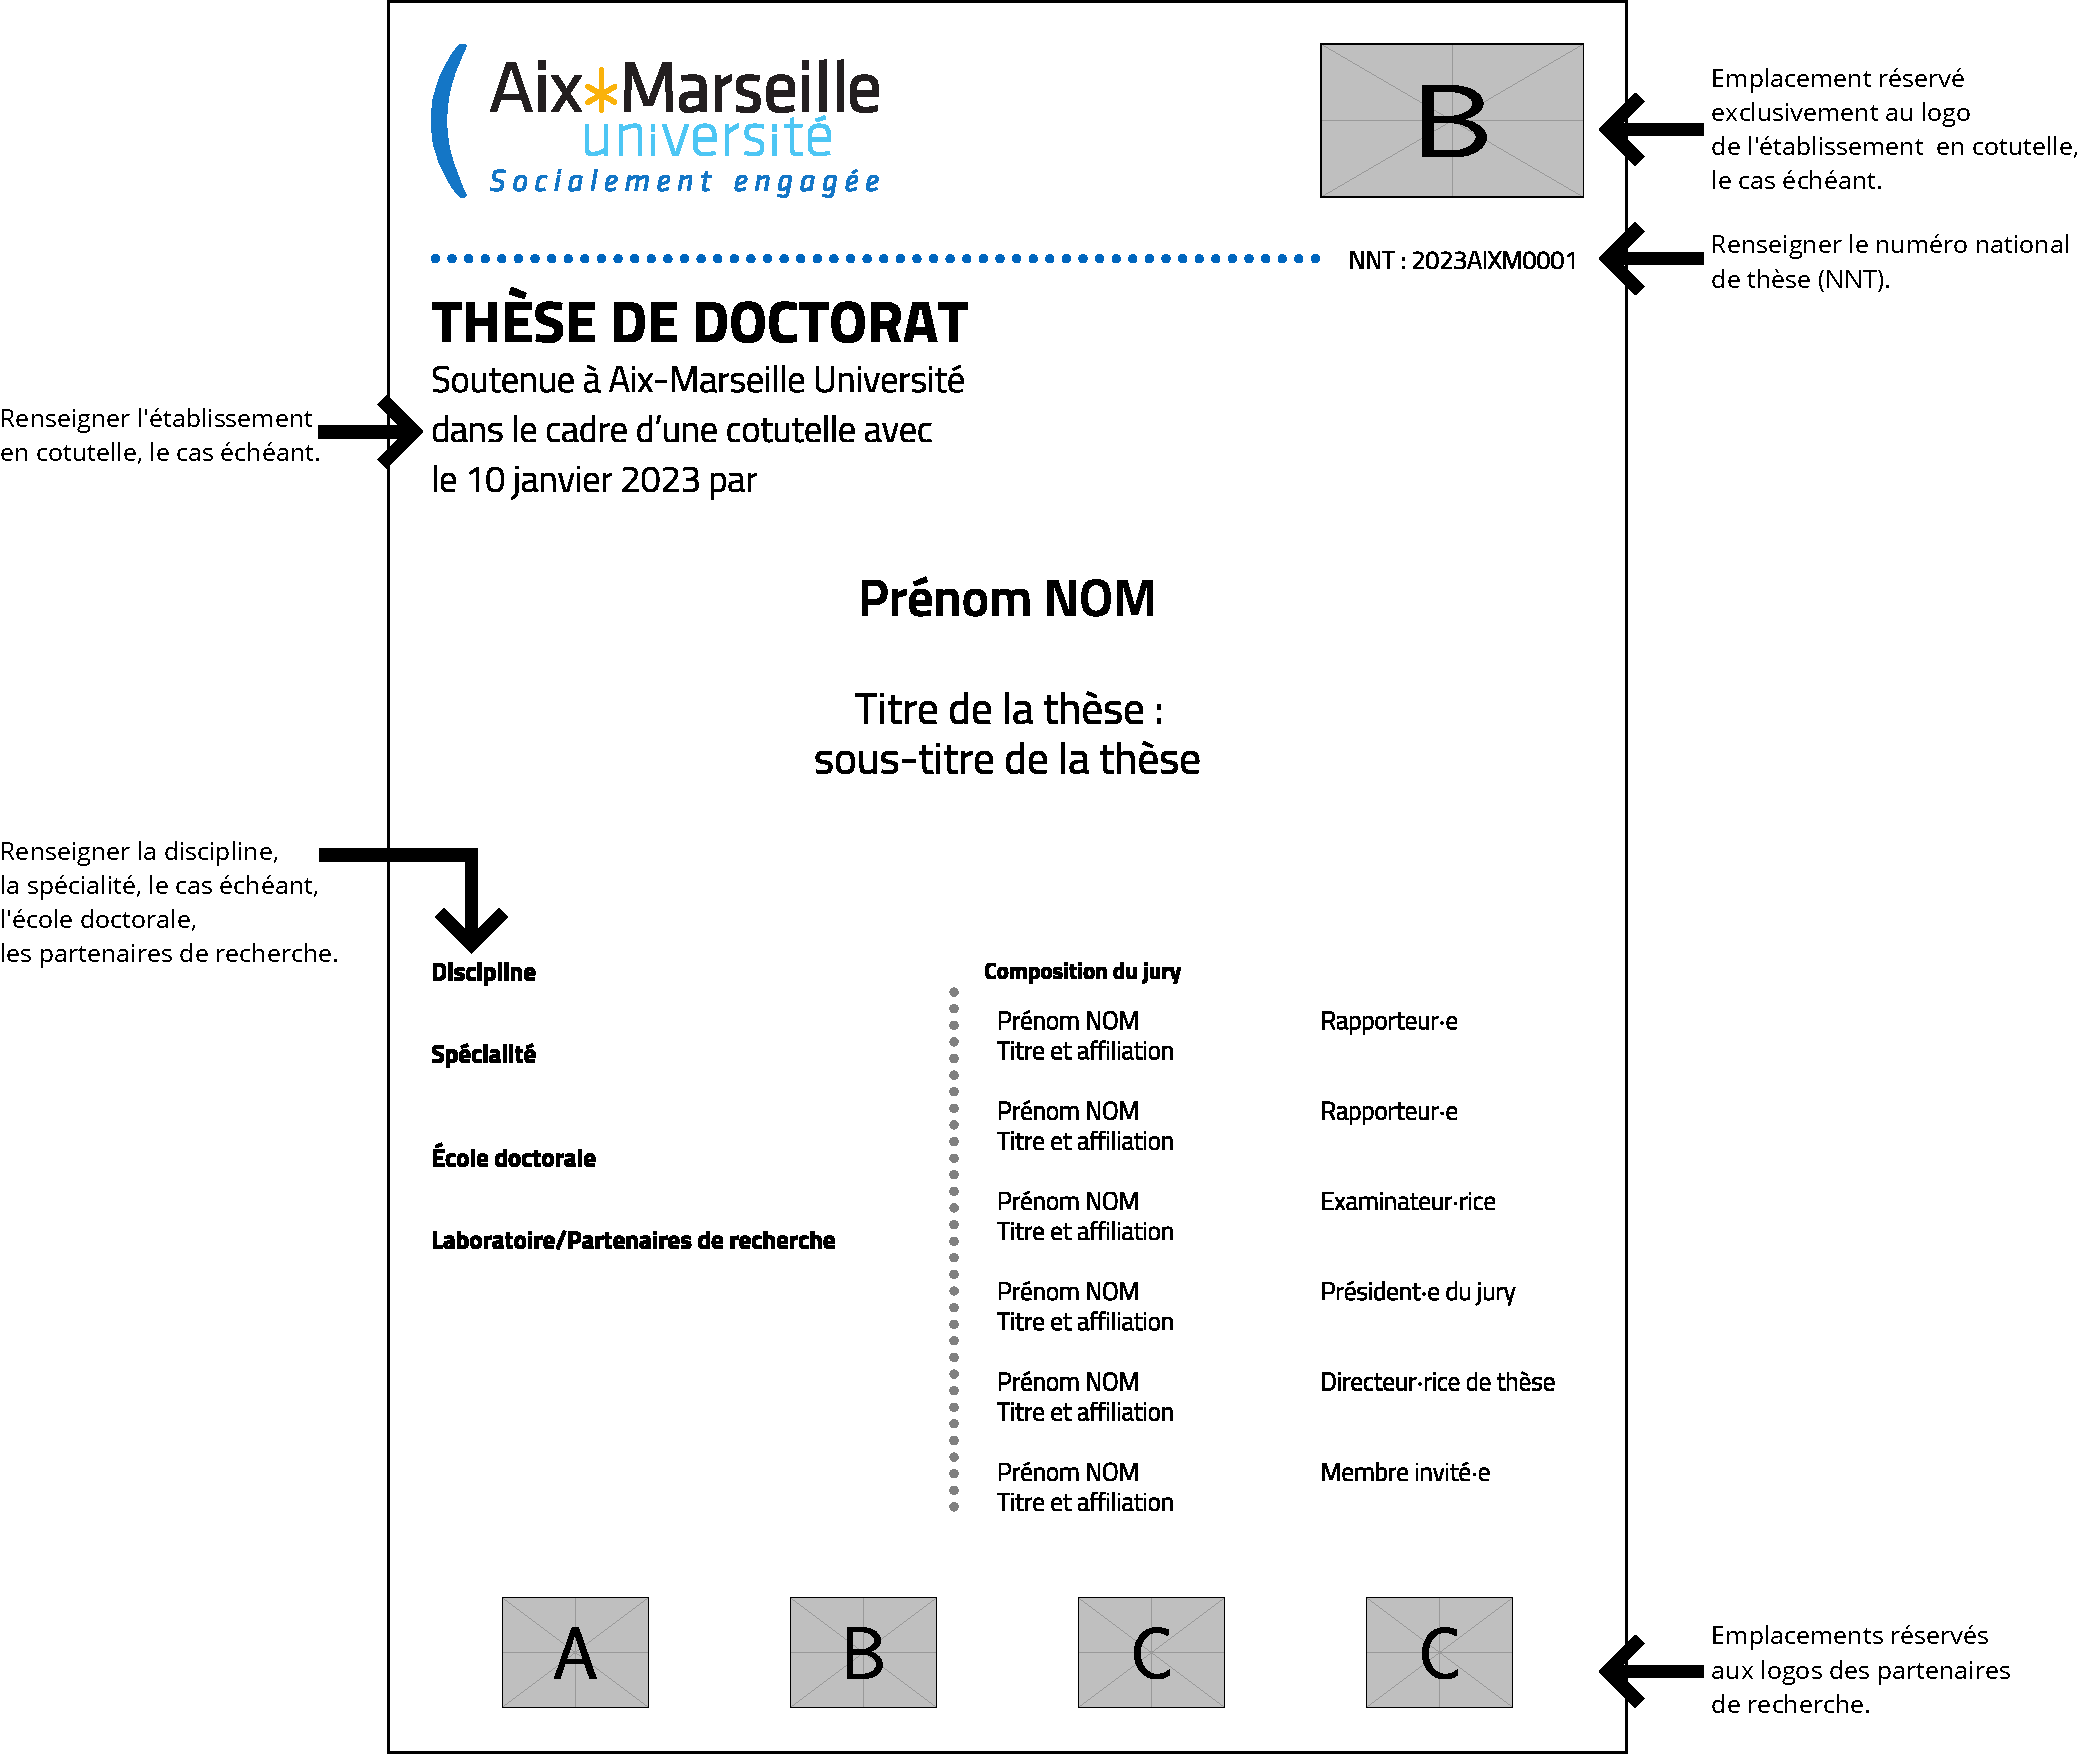
\includegraphics[width=0.8\textwidth]{titre.pdf}
\end{figure}

\begin{itemize}
	\selectlanguage{french}
	\item La page de titre des thèses AMU: elle est rédigée en langue française avec la police Titillium, selon la charte graphique AMU. Elle est fournit avec le modèle LaTeX AMU aux formats TTF et TFM;
	\selectlanguage{english}
	\item The title page of AMU’s thesis: it is written in French with the Titillium font, according to AMU’s graphic charter. It is provided with the LaTeX AMU template in TTF and TFM formats;
	\\

	\selectlanguage{french}
	\item En cas de cotutelle internationale, le logo de l’établissement partenaire doit apparaître en haut à droite de la page de titre;
	\selectlanguage{english}
	\item In the case of international cotutelle, the logo of the partner institution must appear at the top right of the title page;
	\\

	\selectlanguage{french}
	\item La composition du jury, l’école doctorale, la discipline et la spécialité (le cas échéant) doivent être conformes au formulaire ADUM de demande de soutenance de thèse;
	\selectlanguage{english}
	\item The composition of the jury, the doctoral school, the discipline and the specialty (if applicable) must be in accordance with the ADUM application form for the thesis defense;
	\\

	\selectlanguage{french}
	\item Le numéro national de thèse (NNT) doit être apposé sur la page de titre;
	\selectlanguage{english}
	\item The National Thesis Number (NNT) must be displayed on the title page;
	\\
	
	\selectlanguage{french}
	\item Le cas échéant, les logos d’institutions ou d’unité de recherche partenaires peuvent être ajoutés en bas de la page de titre;
	\selectlanguage{english}
	\item Where appropriate, logos of partner institutions or research units can be added to the bottom of the title page;
	\\

	\selectlanguage{french}
	\item La page affidavit: selon la langue utilisée pour la rédaction de de votre thèse, opter pour la version en français ou en anglais, puis la compléter, la dater et la signer;
	\selectlanguage{english}
	\item The affidavit page: according to the language used for writing your thesis, choose the French or English version, then complete, date and sign it;
	\\

	\selectlanguage{french}
	\item La liste des publications réalisées au cours de votre projet de thèse et participation aux conférences durant la même période;
	\selectlanguage{english}
	\item The list of publications made during the course of your thesis project and participation in conferences during the same period;
	\\

	\selectlanguage{french}
	\item Les résumés et mots clés en français et en anglais (un résumé par page): chaque résumé ne doit pas dépasser 1700 caractères;
	\selectlanguage{english}
	\item Summaries and keywords in French and English (one summary per page): each summary must not exceed 1,700 characters.\\
\end{itemize}


\selectlanguage{french}
Selon vos besoins, vous pouvez ajouter les éléments suivants: sommaire et/ou table des matières, liste des figures, liste des tableaux, liste des acronymes, glossaire, index, nomenclature…
Pour le corps de votre thèse, si votre école doctorale ne vous donne pas de consignes plus précises, vous pouvez utiliser les styles établis dans ce modèle ou vos propres styles en suivant ces recommandations:
\begin{itemize}
	\item Police neutre : Il est conseillé d'utiliser une police serif standard pour le texte et une police sans-serif standard pour les titres;
	\item Géométrie : paper=a4, fontsize=12pt, DIV=12;
	\item Interligne simple;
	\item Texte justifié.
\end{itemize}
\selectlanguage{english}
Depending on your needs, you can add the following elements: summary and/or table of contents, list of figures, list of tables, list of acronyms, glossary, index, nomenclature...
For the body of your thesis, if your doctoral school does not give you more specific instructions, you can use the styles established in this template or your own styles following these recommendations:
\begin{itemize}
	\item Neutral font : It is recommended to use a standard serif font for text and a standard sans-serif font for titles;
	\item Geometry : paper=a4, fontsize=12pt, DIV=12;
	\item Single-line spacing;
	\item Justified text.\\
\end{itemize}

\begin{figure}[h!tbp]
	%\vspace{0.5cm}
	\centering
	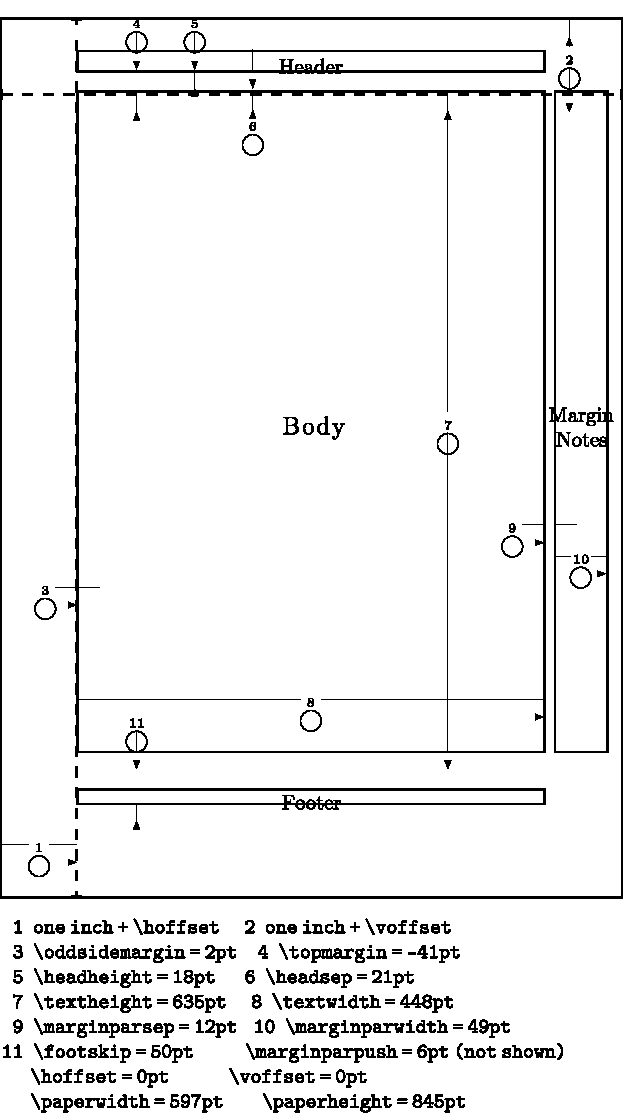
\includegraphics[width=0.4\textwidth]{geometry.pdf}
\end{figure}


\selectlanguage{french}
Votre thèse devra être déposée en ligne en format PDF version 1.5 minimum sur \href{https://www.adum.fr/}{adum.fr}.

\selectlanguage{english}
Your thesis must be submitted online in PDF 1.5 minimum version format on \href{https://www.adum.fr/}{adum.fr}.

